% !TeX spellcheck = da_DK
\documentclass[danish,a4paper,article,12pt]{article}
\documentclass{article}
\usepackage{hyperref}
\usepackage{amsmath}
\usepackage{amssymb}
\usepackage{pgfplots}
\usepackage{float}
\usepackage{todonotes}
\usepackage{tikz}

\renewcommand{\Re}{\mathbb{R}}
\newcommand{\Li}{\mathcal{L}}
\newcommand{\Ex}{\mathbb{E}}
\renewcommand{\Pr}{\mathbb{P}}
\newcommand{\Hy}{\mathcal{H}}

\newcommand\bigO[1]{
    \ensuremath{\mathcal{O}\left(#1\right)}
    }

\newcommand{\sigmoidPlot}{
    
    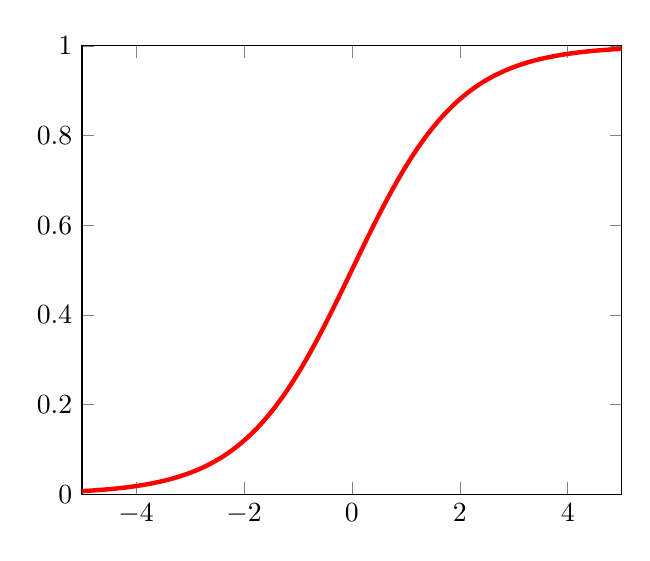
\begin{tikzpicture}
        \begin{axis}[xmin=-5, xmax=5, ymin=0, ymax=1, samples=150]
        \addplot[red, ultra thick] {1/(1+exp(-x))};
        \end{axis}
    \end{tikzpicture}
    
    }

\usetikzlibrary{positioning, calc}
\usetikzlibrary{arrows.meta}

\tikzstyle{circlebox}=[circle,thick,draw=black!75,minimum size=8mm]
\tikzstyle{inputnode}=[circlebox, draw=blue!75]
\tikzstyle{hiddennode}=[circlebox, draw=orange!75]
\tikzstyle{outputnode}=[circlebox, draw=orange!75]
\tikzstyle{simplebox}=[rectangle,thick,draw=black!75,
fill=black!20,minimum size=4mm]
\tikzstyle{textbox}=[rectangle,thick,minimum size=4mm,draw=black!0,
fill=black!0]
\tikzstyle{halfvdistance}=[yshift=-0.7cm]
\tikzstyle{abovebetween}=[xshift=-2.7mm]
\tikzstyle{edgepath} = [-Latex,->,shorten >=1pt,-stealth,semithick, rounded 
corners=5pt]

\def \nodedv {0.735cm}
\def \nodedh {0.65cm}

\tikzset{
    between/.style args={#1 and #2}{
        at = ($(#1)!0.5!(#2)$)
    }
}

\title{P, NP and NPC}
\author{Lukas Jørgensen, 201206057
	}
\date{\today}

\begin{document}

\maketitle

\section{Disposition}
\begin{itemize}
\item Hvilke problemer - Beslutningsproblemer, encoding
\item Hvad er et sprog
\item Hvad er et stand-in problem
\item P og NP
\item Reduktioner
\item NPH og NPC
\end{itemize}

\section{Noter}

\subsection{Problemer}
Problemer kan være hvad som helst, alt fra 2+2 til "hvordan farver jeg denne graf med 3 farver".

I dette kursus har vi begrænset os til at se på beslutningsproblemer, det vil sige problemer hvor outputtet altid er "ja" eller "nej" instanser. Dette kan også beskrives ved binære strenge over $\{0,1\}$. Grunden til dette er, at vi da kan opfatte problemerne som "sprog" hvor der gælder at:
\begin{equation}
x\in L \text{ iff $x$ er en "ja" instans til problemet.}
\end{equation}

Udover at begrænse typen af problemer, har vi også valgt at begrænse os til at se på inputs der er bitstrenge over $\{0,1\}^*$. Selvom vi har denne begrænsning, er vores inputs stadig meget generelle, da dette allerede gøres i computere, hvor man f.eks. kan encode tekst v.h.a. ASCII. Ethvert naturligt tal kan da encodes i binære bitstrenge, sådan som det allerede gøres i computere, de kan dog ikke repræsentere reelle tal.

\subsection{Stand-in problemer}
For at vise at restriktionen med at vi kun kigger på beslutningsproblemer, stadig er ret generel, kigger vi på såkaldte stand-in problemer. Disse stand-in problemer er beslutningsproblemer der kan bruges til at løse\todo{Tjek dette} de egentlige problemer.

\subsubsection{Problemer med bitstrenge som output}
Hvis vi har nogle problemer hvor outputtet ikke består af "ja" eller "nej", men i stedet består af en arbitrær bitstreng, kan vi konstruerer et stand-in sprog for dette problem.

Et stand-in sprog for en given funktion $f:\{0,1\}^* \rightarrow \{0,1\}^*$ kan skrives således:
\begin{equation}
L_f = \{\langle x,b(j),y \rangle |f(x)_j=y\}
\end{equation}
Således kan man udregne outputtet en bit ad gangen.

\subsubsection{Optimeringsproblemer}
Hvis vi har givet et optimerings problem:

\begin{quote}
\textbf{OPT:} “Givet en inputstreng der definerer et sæt mulige løsninger
$F$ og en objective funktion $f$, find $x\in F$ der maksimerer
$f(x)$”.
\end{quote}
a
Dette er dog ikke et beslutningsproblem, og vi (tror) ikke at vi kan tjekke det i polynomiel tid. I stedet kan vi udtrykke dette problem som et beslutningsproblem vha. følgende stand-in sprog:

\begin{quote}
$\mathbf{L_{OPT}}$: “Givet en inputstreng der definerer $F$, $f$ og en target
værdi $v \in Q$, bestem hvorvidt der er en løsning $x \in F$ således
$f(x) \geq v$”.
\end{quote}

Dette er dog ikke en perfekt "stand-in" da $L_{OPT}$ sagtens kan have en effektiv løsning, uden at $OPT$ har det. Omvendt, kan så ved vi at hvis $L_{OPT}$ er svær at løse, så ved vi også at $OPT$ er det. (Hvis vi kan finde den maksimale værdi i polynomiel tid, kan vi også bestemme hvorvidt der er en løsning der større end $v$ i polynomiel tid.)

Derfor kan vi ikke bruge $L_{OPT}$ til at vise at et problem har en effektiv løsning, men vi kan bruge det til at argumentere for at et givent problem er svært.

\subsection{P og NP}

\begin{figure}
\centering
\includegraphics{NP-CompleteSet.png}
\caption{En figur der visualiserer P, NP, NPC og NP-Hård}
\end{figure}

\subsubsection{P}
Kompleksitetsklassen $P$ er klassen af beslutningsproblemer, der kan blive bestemt af en deterministisk Turing Maskine, hvor antallet af "steps" maskinen udfører for et eller andet input $x$ er $\rho(x)$ for et arbitrært polynomie $\rho$. Dvs. det er polynomielt i inputtet. 

Dette kan også beskrives som ethvert problem med worst-case kørselstid $O(n^k)$ for et givent $k$.

Formelt defineres $P$ som:
\begin{equation}
P= \{L\subseteq \{0,1\}^* | \exists \text{ TM} \, M_L \text{ der afgører L i polynomiel tid.} \}
\end{equation}

Det skal dog siges, at i praksis kan man godt komme ud for at et teoretisk "svært" problem, godt kan være lettere end et teoretisk "let" problem. Når man ser på problemerne teoretisk, tager man ikke højde for konstanter eller forventet kørselstid som kan betyde at et problem kan være lettere at løse i de praktiske tilfælde frem for det rent teoretiske.

\subsubsection{NP}
Kompleksitetsklassen $NP$ klassen af beslutningsproblemer for hvilket "ja" instanserne kan verificeres i polynomiel tid. Altså, tager løsningen til disse problemer eksponentiel tid, men man kan verificere en given løsning til problemet i polynomiel tid.

Formelt defineres $NP$ således:
\begin{equation}
\forall x: \, x\in L \Leftrightarrow \{\exists y \in \{0,1\}^* : |y| \leq \rho(|x|) \wedge \langle x,y \rangle \in L' \}
\end{equation}

Denne definition kan forstås således: vi har et instans af et problem $x\in L$, vi har da sættet af binære strenge med længde $\leq \rho(|x)$ der repræsenterer potentielle løsninger til problemet der er associeret med instansen $x$. Med denne fortolkning, betyder $\langle x,y \rangle \in L'$ at den potentielle løsning $y$ er en korrekt løsning til problemet. 

\subsection{Reduktioner}

\subsubsection{Polynomial time computable maps}
Et polynomial time computable map, er en funktion $f:\{0,1\}^* \rightarrow \{0,1\}^*$, hvor der gælder at:
\begin{equation}
\forall x: |f(x)| \leq \rho(|x|)
\end{equation}
\begin{equation}
L_f \in P
\end{equation}
For et arbitrært polynomium $\rho$.

D.v.s at længden af funktionens output er polynomielt på inputtet og sproget for funktionen $f$ skal have en polynomiel kørselstid.

Dette kan også ses som en måde at oversætte fra en repræsentation eller model, til en anden i polynomiel tid, vha. en funktion $f$.

\subsubsection{Polynomielt ækvivalente repræsentationer}
To repræsentationer $\pi_1$ og $\pi_2$ er polynomielt ækvivalente hvis der findes polynomial time computable maps $r_1$ og $r_2$ der oversætter mellem de to repræsentationer.

D.v.s. for alle $x\in S$ hvor $S$ er instanserne for et beslutningsproblem $f:S\rightarrow \{yes,no\}$ (f.eks. sættet af all endelige directed graphs).
\begin{equation}
\pi_1(x)=r_1(\pi_2(x)) \wedge \pi_2(x)=r_2(\pi_1(x))
\end{equation}

\subsubsection{Reduktioner}
Vi siger at $L_1$ \emph{reducerer til} $L_2$ ($L_1 \leq L_2$) hvis der er en polynomial time computable funktion $r$ således at for alle $x\in \{0,1\}^*$ så har vi at $x\in L_1 iff r(x)\in L_2$.

\subsection{NP-Hard og NPC}

\subsubsection{NP-hard}
Et sprog er \texttt{NP-hard} hvis der gælder:
\begin{equation}
\forall L' \in \text{ NP } : L' \leq L
\end{equation}

Altså gælder der, at ethvert sprog $L'$ i NP kan reduceres til $L$. Altså er algoritmen til at løse \texttt{NP-hard} problemet så generel, at den kan bruges til at løse ethvert andet problem i NP. Derfor siger man også at det intuitivt set er mindre sandsynligt at et \texttt{NP-hard} problem er i $P$, da det vil medføre at $P=NP$.

NP-hard problemer er ikke nødvendigvis i $P$, og hvis de er i $P$ kaldes de typisk \texttt{NP-Complete} i stedet.

\subsubsection{NPC}
\texttt{NP-Complete} (NPC) er den klasse af problemer der både er \texttt{NP-hard} og ligger i NP. Vi kan definerer dette formelt således:

\begin{equation}
\text{NPC}=\{ L\in \{0,1\}^* \| L\in NP \wedge (\forall L' \in \text{NP} : L' \leq L) \}
\end{equation}

NPC-problemer er interessante, fordi vi kan ved hjælp af disse problemer, bevise at et givent problem ikke ligger i $P$ medmindre $P=NP$ og derved undgå at bruge tid på at forsøge at finde en algoritme i $P$ til et problem der (formentlig) ikke har en effektiv løsning.

\section{Beviser}

\subsection{Proposition 3 - transitivitet af reduktioner}
\emph{Hvis $L_1 \leq L_2$ og $L_2 \leq L_3$ så gælder der at $L_1 \leq L_2$} (transitivitet af reduktioner).

Da $L_1 \leq L_2$ og $L_2 \leq L_3$ så ved vi at vi har to polynomial time computable maps $r_1$ og $r_2$, hvor der gælder:

\begin{itemize}
\item For ethvert arbitrært $x$ er $x\in L_1$ iff $r_1(x) \in L_2$
\item For ethvert arbitrært $y$ er $y\in L_2$iff $r_2(x) \in L_3$
\end{itemize}

Heraf kan vi så se at for alle $x$, har vi at $x \in L_1$ iff $r_2(r_1(x)) \in L_3$. Da vi blot bruger to polynomial time computable maps efter hinanden, vil det tage $\rho_1(|x|)+\rho_2(|r_1(x))$ tid, hvilket stadig er polynomielt så derfor har vi at $L_1 \leq L_3$.

\subsection{Proposition 5 - $\text{NP-hard} \in P \implies P=NP$}
\emph{Lad $L$ være et NP-hard sprog. Hvis $P\neq NP$ så gælder der at $L\notin P$}

Siden $L$ er \texttt{NP-Hard}, gælder der at $\forall L' \in NP: L' \leq L$. Hvis vi derimod antager at $L\in P$ så gælder der at alle $L'\in NP$ er i $P$ og derfor gælder det at $P=NP$.

\subsection{Proposition 6}
\emph{Lad $L \in NPC$ så er $P=NP$ iff $L\in P$}

Fra proposition 5 ved vi at $P\neq NP$ hvis $L\notin P$, men vi ved ikke direkte herfra at det er "hvis og kun hvis".

Vi kan derimod udlede dette fra at $L\in NP$. Da vi fra proposition 5 ved at $L\notin P$ og vi ved at sproget er i $NP$, så må det betyde at $P\neq NP$ iff $L\notin P$ og derved at $P=NP$ iff $L\in P$.

\end{document}